\documentclass{article}
\usepackage{graphicx} % Required for inserting images

\title{Problem Set 9}
\author{https://github.com/kdindial/phys-ga2000}
\date{November 2024}

\begin{document}

\maketitle

\section{Problem 1}
We start with a very exciting second order differential equation:
\begin{equation}
    \frac{d^2x}{dt^2}=-w^2x(t)
\end{equation}

And are asked to turn it into two coupled first order equations:
\begin{equation}
    \frac{dx}{dt}=v(t)
\end{equation}

\begin{equation}
    \frac{dv}{dt}=-w^2x(t)
\end{equation}

Then we are asked to set make a plot of x as a function of time with omega equal to 1 and initial conditions. I made an rk4 integrator with fixed time steps and made a plot of displacement versus time for $\omega$ equal to 1, initial velocity=0 and initial position equal to 1 over a time interval of 50 seconds. Next had the rk4 integrator solve for the motion of the SHO with an initial xvalue of 2 and velocity of 0 and plotted the two over eachother to show that the period of oscillation was roughly the same
\begin{figure}
    \centering
    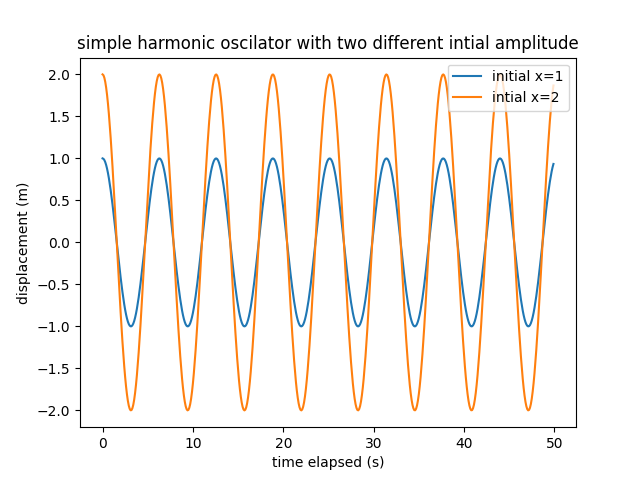
\includegraphics[width=0.8\linewidth]{8_6_b.png}
    \caption{Problem 1 parts a and b}
    \label{fig:1}
\end{figure}

Next we are asked to change our second order ODE to an anharmonic oscilator. In this case:


    \begin{equation}
    \frac{d^2x}{dt^2}=-w^3x(t)
    \end{equation}

I plotted x position vs time with 3 different initial positions of x as shown in fig 2.

\begin{figure}
    \centering
    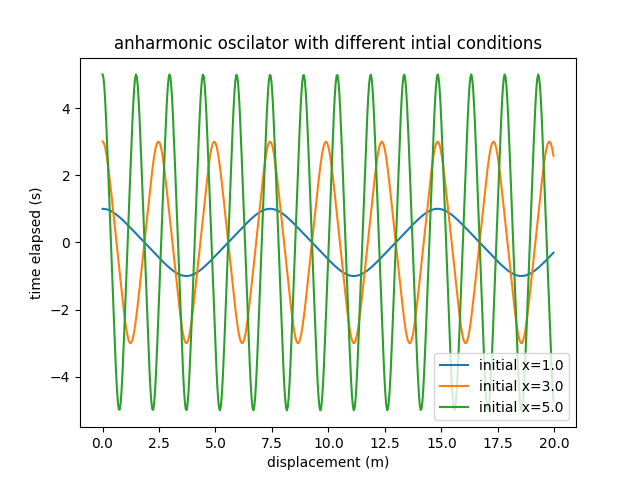
\includegraphics[width=0.8\linewidth]{aho.png}
    \caption{Anharmonic oscilator}
    \label{fig:2}
\end{figure}

When the amplitude is larger, the frequency is faster.

We can also look at the phase space plots of the anharmonic oscillator and the simple harmonic oscillator. Usually phase space plots position vs momentum, but in this case we are going to just plot position vs displacement

\begin{figure}
    \centering
    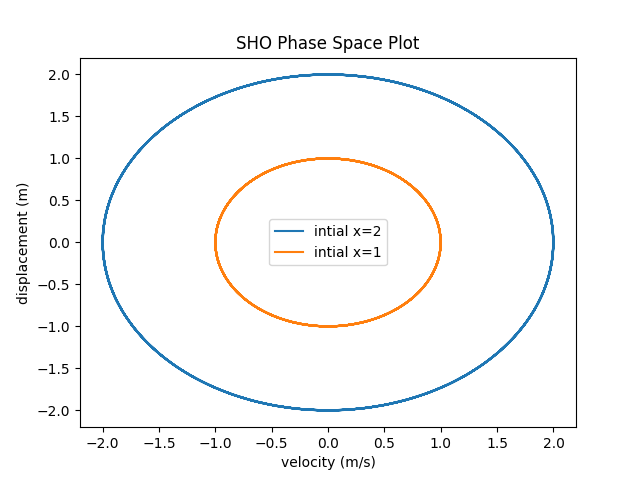
\includegraphics[width=0.8\linewidth]{sho_phase.png}
    \caption{SHO Phase Space}
    \label{fig:3}
\end{figure}

\begin{figure}
    \centering
    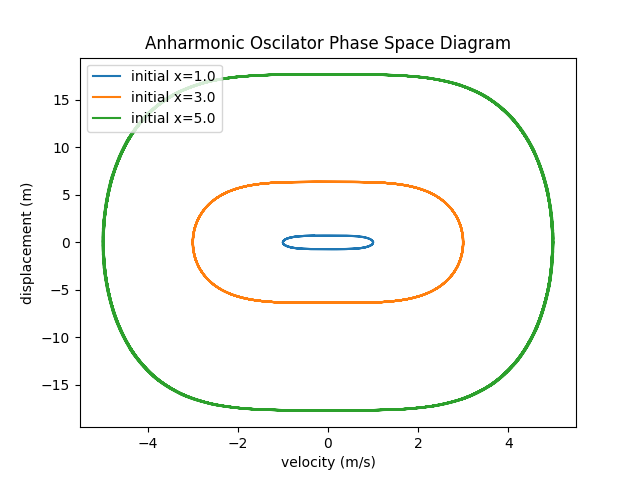
\includegraphics[width=0.8\linewidth]{aho_phase.png}
    \caption{AHO Phase Space}
    \label{fig:4}
\end{figure}


As expected, the SHO makes elipses in phase space with larger elipses corresponding to larger energies. The anharomnic oscilator on the other hand does not make elipses. I am not really sure what to call that shape.

Lastly, we look at the phase space plot for a van der Pol oscillator. Its equation of motion is:
\begin{equation}
    \ddot{x}-\mu(1-x^2)\dot{x}+\omega^2 x=0
\end{equation}
I plugged this equation into my rk4 integrator and got the following phase space plot:

\begin{figure}
    \centering
    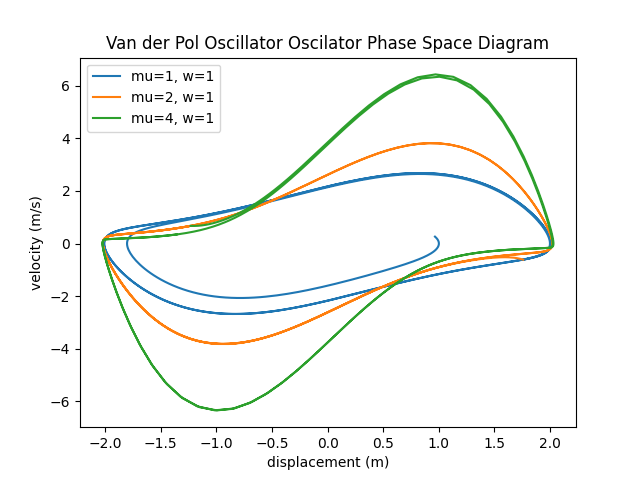
\includegraphics[width=0.8\linewidth]{vdp_phase.png}
    \caption{VPD Oscillator Phase Space}
    \label{fig:enter-label}
\end{figure}
It appears that the phase space plot does not make a closed curve, so either the motion is not periodic or its period is longer than 20s


\section{Problem 2}

We start with the differential equations for a spherical mass subject to  a constant gravitational field and air resistance. In the x direction, we have:

\begin{equation}
    \frac{d^2x}{dt^2}=-\frac{\pi R^2 C\rho}{2m}\dot{x}\sqrt{\dot{x}^2+\dot{y}^2}
\end{equation}

and in the y direction:
\begin{equation}
    \frac{d^2y}{dt^2} =-g- \frac{\pi R^2C\rho}{2m} \dot{y}\sqrt{\dot{x}^2+\dot{y}^2}
\end{equation}

First we are asked to rescale time to a unit-less t' where 
\begin{equation}
    t'=t \sqrt{\frac{R^2 \rho g C}{m}}
\end{equation}

We are also asked to rescale x' to something unit-less, so I decided:

\begin{equation}
    x'=x/R
\end{equation}

We can now rescale our first and second time derivatives:

\begin{equation}
    \frac{dx}{dt}=\frac{dx'}{dt'}R\sqrt{\frac{\rho g C}{m}}
\end{equation}

and
\begin{equation}
    \frac{d^2x}{dt^2}=\frac{d^2x'}{dt'^2}(\frac{R^3 \rho g C}{m})
\end{equation}


plugging in our rescaled equations into the two original equations:

\begin{equation}
    \ddot{x'}=-\frac{\pi R^3 C}{2m}\dot{x'}\sqrt{\dot{x'^2}+\dot{y'}^2}
\end{equation}
\begin{equation}
    \ddot{y'}=-\frac{m}{R^3 \rho C}-\frac{\pi R^3 C}{2m}\dot{y'}\sqrt{\dot{x'}^2+\dot{y'}^2}
\end{equation}

Clearly now we can substitute $\frac{R^3 \rho C}{m}$ for a  unitless paramater called K or something:

\begin{equation}
    \ddot{x'}=-\frac{\pi}{2}K\dot{x'}\sqrt{\dot{x'}^2+\dot{y'}^2}
\end{equation}
\begin{equation}
    \ddot{y'}=-\frac{1}{K}-\frac{\pi}{2}K\dot{y'}\sqrt{\dot{x'}^2+\dot{y'}^2}
\end{equation}


Now we can use this equation for our rk4 integrator, but we also have to remember to rescale all our positions, velocities and times to unit less parameters, then scale them back when plotting. 

\begin{figure}
    \centering
    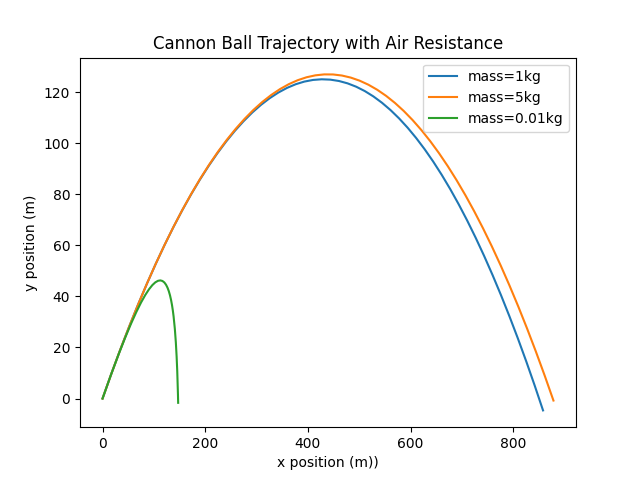
\includegraphics[width=0.8\linewidth]{trajectories.png}
    \caption{Cannon ball trajectories}
    \label{fig:enter-label}
\end{figure}
Using the parameters from the newman problem, the 1kg cannon ball travels horizontally for 858 meters, the 0.01kg cannon ball travels for 147 meters and the 5kg cannon ball travels 878m.

\end{document}